\chapter{生殖的激素调控}\label{ch:b2:reproductive-hormones}

三十年间，每月的节律误差保持在一两天之内：
一个\omterm{def:b2:mammal-reproduction:ovary}{卵泡}成熟，一枚卵子排出，\omterm{def:b2:reproductive-hormones:cycle}{子宫内膜}增厚，
若无胚胎\omterm{def:b2:mammal-reproduction:implantation}{着床}，则随之脱落。
体内没有任何时钟以这一速率运行；这一节律源于
三个器官之间的“对话”——下丘脑、
垂体与卵巢。在此对话中，每种激素调控下一种激素的释放，
而最后一种又调控第一种。本章
将拆解这一“对话”：两性共有的轴、
\omterm{def:b2:mammal-reproduction:testis}{睾丸}的持续性调控、卵巢的周期性调控，
及卵巢由负反馈向正反馈的显著转换，
以及妊娠、药物与临床干预
改写这一轴的方式。

\section{轴}

\begin{definition}[下丘脑-垂体-性腺轴]\label{def:b2:reproductive-hormones:axis}
\index{促性腺激素释放激素}\index{黄体生成素}\index{卵泡刺激素}\index{负反馈!激素性}
\emph{下丘脑}的神经元分泌\emph{GnRH}
（促性腺激素释放激素，一种由十个氨基酸组成的肽）释放入
通往\emph{垂体前叶}的微小门脉血管，
以每一至两小时一次的短暂\emph{脉冲}释放。GnRH 促使
垂体向全身血液循环分泌两种糖蛋白激素，
即\emph{促性腺激素}\emph{LH}（\omterm{def:b2:mammal-reproduction:ovary}{黄体}生成素）
与\emph{FSH}（\omterm{def:b2:mammal-reproduction:ovary}{卵泡}刺激素），二者作用于
\emph{性腺}：LH 作用于产生类固醇的细胞（\omterm{def:b2:mammal-reproduction:testis}{莱迪希细胞}、
\omterm{def:b2:mammal-reproduction:ovary}{卵泡}膜细胞与\omterm{def:b2:mammal-reproduction:ovary}{黄体}细胞），FSH 作用于滋养配子的细胞（
\omterm{def:b2:mammal-reproduction:testis}{支持细胞}与颗粒细胞）。性腺以类固醇作出应答——
\emph{睾酮}、\emph{雌二醇}、\emph{孕酮}——以及
多肽\emph{抑制素}，这些物质反馈作用于
下丘脑和垂体：类固醇对二者多为
\emph{负向}作用；抑制素仅作用于 FSH。由此形成一个受调节的
环路，性腺的输出维持在调定点，
相同的三级结构也调控甲状腺和肾上腺皮质。这些激素作用于靶细胞的
机制将在
\cref{ch:b2:cell-signalling}中讨论。
\end{definition}

\begin{omfigure}
\begin{tikzpicture}[every node/.style={font=\scriptsize}, >=stealth]
  \node[draw, rounded corners, fill=omDef!15, align=center, minimum width=3cm] (hyp) at (0,4.2) {下丘脑 \\GnRH，脉冲式};
  \node[draw, rounded corners, fill=omDef!15, align=center, minimum width=3cm] (pit) at (0,2.2) {垂体前叶 \\LH 与 FSH};
  \node[draw, rounded corners, fill=omProp!20, align=center, minimum width=3cm] (gon) at (0,0) {性腺 \\类固醇、抑制素};
  \node[draw, rounded corners, fill=omExo!25, align=center, minimum width=3cm] (tar) at (5.2,0) {靶组织 \\配子发生、导管、\\第二性征};
  \draw[->, thick] (hyp) -- (pit) node[midway, right] {门脉血管};
  \draw[->, thick] (pit) -- (gon) node[midway, right] {血液};
  \draw[->, thick] (gon) -- (tar);
  \draw[->, thick, omThm] (gon.west) .. controls (-3.0,0) and (-3.0,2.2) .. (pit.west);
  \draw[->, thick, omThm] (gon.west) .. controls (-4.6,0) and (-4.6,4.2) .. (hyp.west);
  \node[omThm, anchor=east, align=right] at (-3.9,1.2) {对垂体：\\类固醇 $(-)$，\\抑制素 $(-)$ 作用于 FSH};
  \node[omThm, anchor=east, align=right] at (-3.9,3.6) {对下丘脑：\\类固醇 $(-)$\\（雌二醇 $(+)$\\于周期中期）};
\end{tikzpicture}

{\small 轴：下丘脑 GnRH 驱动垂体 LH 与 FSH，
二者驱动性腺；性腺分泌的类固醇与抑制素
对两个上级环节起负反馈作用——唯触发\omterm{def:b2:mammal-reproduction:ovary}{排卵}的
雌二醇所引起的短暂正反馈例外。}
\end{omfigure}

\begin{proposition}[脉冲为何重要]\label{prop:b2:reproductive-hormones:pulses}
\index{脉冲式分泌}\index{受体脱敏}
垂体只有在 GnRH 以脉冲形式到达时才会作出反应。细胞
持续暴露于某种激素时，细胞会移除表面的该激素受体
（\emph{脱敏}）；若受体池以速率 $s$ 补充、
以基础速率 $d$ 移除，在
激素 $H$ 存在时还以附加速率 $iH$ 移除，则
\[
\frac{\mathrm{d}R}{\mathrm{d}t} = s - (d + iH)\,R, \qquad R^* = \frac{s}{d + iH},
\]
因此持续的高浓度 $H$ 使受体数量降至较低的
稳态，细胞随之“沉默”，而短暂的脉冲
被无激素的间隔分隔开来，使受体池在其间得以恢复
（时间常数 $1/d$）。每九十分钟一次的 GnRH 脉冲
可维持垂体的反应性；持续灌注或
长效 GnRH 激动剂则在数天内使其失效——这正是
用于抑制前列腺癌、\omterm{def:b2:reproductive-hormones:cycle}{子宫内膜}异位症
和性早熟的药物的基础。脉冲频率也携带信息：
快速脉冲有利于 LH，慢速脉冲有利于 FSH。
\end{proposition}
\begin{proof}[证据]
克诺比尔（1978--1980）破坏了恒河猴的 GnRH 神经元，
导致 LH、FSH 及周期均消失，随后以泵替代
GnRH 给药：每小时一次脉冲恢复了促性腺激素和正常的
\omterm{def:b2:mammal-reproduction:ovary}{排卵}周期；同样的日剂量若持续给予，
仅恢复数天，随后 LH 与 FSH 降至零；
改回脉冲给药后，又得以恢复。起作用的是给药
模式，而非剂量。
\end{proof}

\begin{omfigure}
\begin{tikzpicture}
\begin{axis}[
  width=0.8\linewidth, height=5.4cm,
  axis x line=bottom, axis y line=left,
  xmin=0, xmax=40, ymin=0, ymax=1.2,
  xlabel={天}, ylabel={血浆 LH（相对值）},
  xlabel style={font=\small, at={(axis description cs:0.5,-0.13)}, anchor=north},
  ylabel style={font=\small},
  tick label style={font=\small}, xtick={0,10,20,30,40}, ytick={0,0.5,1},
  clip=false,
]
\addplot[very thick, omDef, domain=0:10, samples=2] {1};
\addplot[very thick, omThm, domain=10:25, samples=60] {exp(-(x-10)/3)};
\addplot[very thick, omDef, domain=25:40, samples=60] {1-exp(-(x-25)/2)};
\fill[omDef!15] (axis cs:0,1.05) rectangle (axis cs:10,1.15); \node[font=\scriptsize] at (axis cs:5,1.1) {每小时一次脉冲};
\fill[omThm!15] (axis cs:10,1.05) rectangle (axis cs:25,1.15); \node[font=\scriptsize] at (axis cs:17.5,1.1) {持续灌注};
\fill[omDef!15] (axis cs:25,1.05) rectangle (axis cs:40,1.15); \node[font=\scriptsize] at (axis cs:32.5,1.1) {再次脉冲};
\end{axis}
\end{tikzpicture}

{\small 克诺比尔的实验示意。在一只自身的
GnRH 神经元被破坏的猴子中，每小时一次的 GnRH 脉冲维持 LH；
改为持续输注等量的日剂量，
数日内 LH 即消失，而脉冲式给药可使其恢复。}
\end{omfigure}

\begin{omfigure}
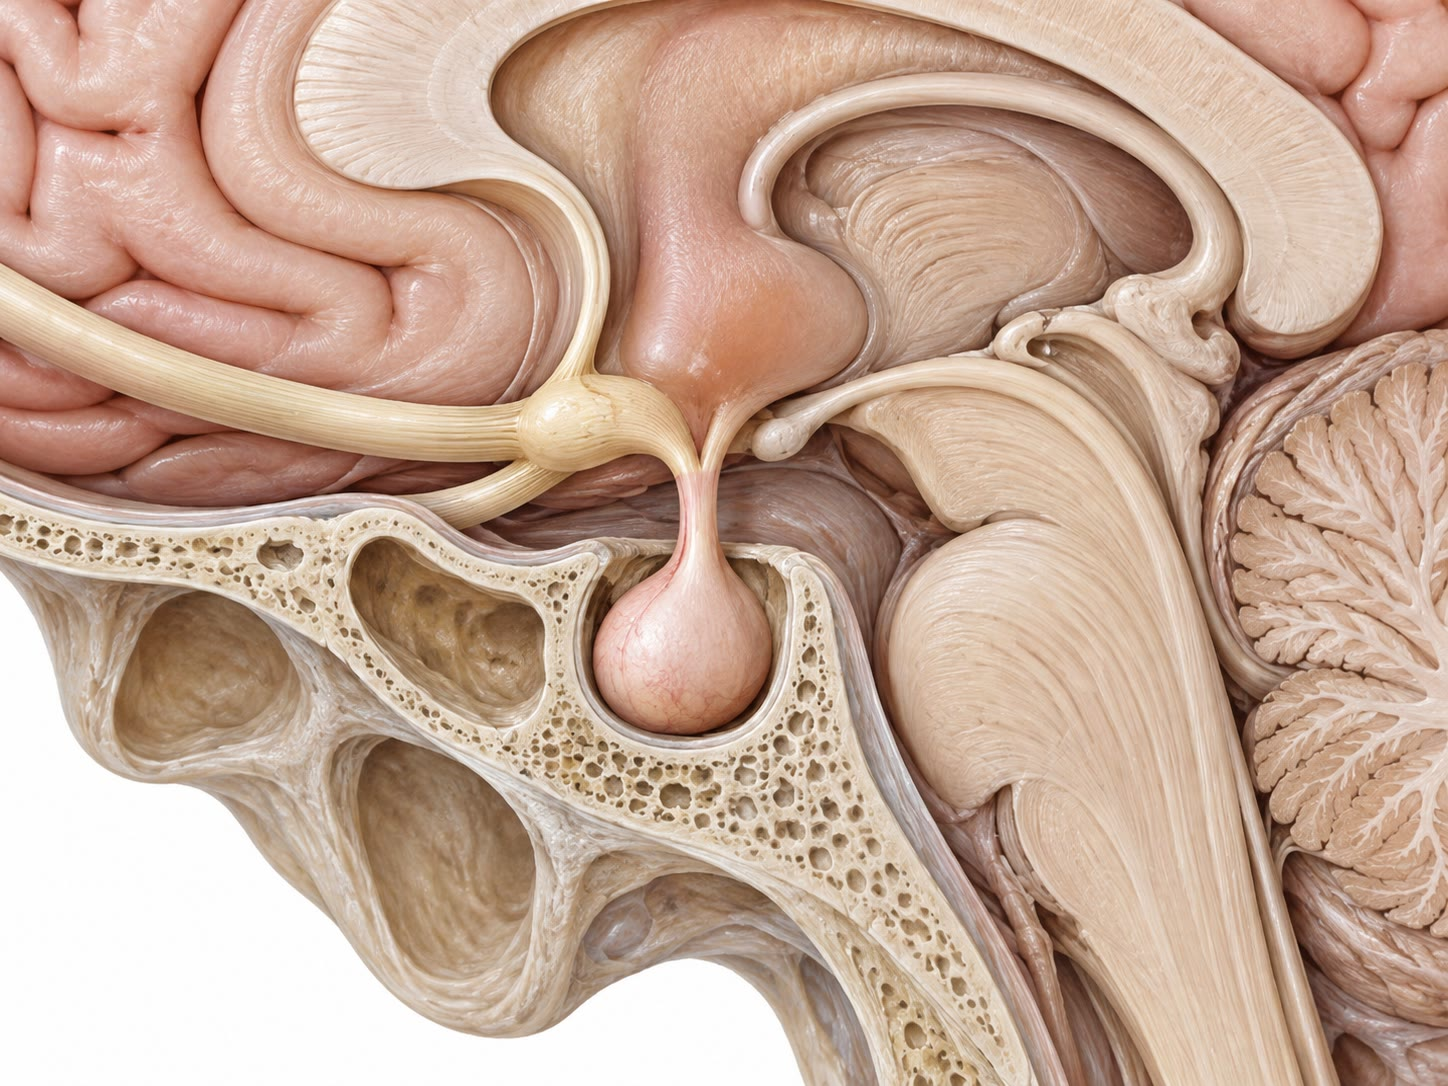
\includegraphics[width=0.55\linewidth]{images/book4/ai/b4-09-hypothalamus-pituitary.jpg}

{\small 矢状切面所示的脑底：下丘脑
位于上方，垂体柄居中，垂体位于骨性的垂体窝中——
即该轴的“硬件”。}
\end{omfigure}

\section{男性：紧张性调控}

\begin{proposition}[睾丸的调控]\label{prop:b2:reproductive-hormones:testis}
\index{睾酮}\index{抑制素}
LH 作用于\omterm{def:b2:mammal-reproduction:testis}{莱迪希细胞}，后者分泌\emph{睾酮}
（成年男性血液中为 \qtyrange{3}{10}{ng/mL}，\omterm{def:b2:mammal-reproduction:testis}{睾丸}内则高出约一百
倍）。FSH 作用于\omterm{def:b2:mammal-reproduction:testis}{支持细胞}，\omterm{def:b2:mammal-reproduction:testis}{支持细胞}
在局部睾酮的配合下支持\omterm{def:b2:mammal-reproduction:testis}{精子发生}，并分泌
\emph{抑制素}。睾酮对下丘脑
和垂体进行反馈以抑制 LH；抑制素对垂体进行反馈，
以抑制 FSH。两条回路均为\emph{负}反馈，而系统为
\emph{紧张性}的：激素水平随脉冲与
昼夜变化（清晨最高），但不呈周期性；精子则持续产生。
睾酮还促进并维持附属腺体和导管、
胡须、嗓音、肌肉与骨骼、红细胞生成及性欲，
并在胎儿期使男性躯体得以形成
（见\cref{ch:b2:mammal-reproduction}）。去势后睾酮消失：
LH 和 FSH 因失去反馈而升高数倍，次级性征
随之退化；注射睾酮可使性征恢复，
但不能恢复生育力，因为睾酮同时抑制 LH，
从而降低\omterm{def:b2:mammal-reproduction:testis}{精子发生}所需的\omterm{def:b2:mammal-reproduction:testis}{睾丸}内睾酮。这正是
合成类固醇使男性不育的原因。
\end{proposition}
\begin{proof}[证据]
贝特霍尔德（1849 年）阉割公鸡，鸡冠萎缩，它们
既不啼鸣，也不争斗。将\omterm{def:b2:mammal-reproduction:testis}{睾丸}移植到去势
个体的腹腔中，\omterm{def:b2:mammal-reproduction:testis}{睾丸}长出了新的血液供应却无神经，使
鸡冠、啼鸣与争斗得以恢复：\omterm{def:b2:mammal-reproduction:testis}{睾丸}是通过血液发挥作用的——
这是首次证明内分泌物的存在，早于“激素”一词
约五十年。睾酮于 1935 年被分离并合成。
\end{proof}

\section{女性：一个带开关的循环}

\begin{definition}[卵巢循环与子宫循环]\label{def:b2:reproductive-hormones:cycle}
\index{月经周期}\index{卵泡期}\index{黄体期}\index{LH 峰}\index{子宫内膜}
循环自月经第一天起算，持续
约 28 天。\emph{\omterm{def:b2:mammal-reproduction:ovary}{卵泡}期}（第 1--14 天）：FSH
因前一\omterm{def:b2:mammal-reproduction:ovary}{黄体}退化而摆脱反馈抑制，募集了一批
\omterm{def:b2:mammal-reproduction:ovary}{卵泡}；\omterm{def:b2:mammal-reproduction:ovary}{卵泡}分泌\emph{雌二醇}，其水平稳步上升；
雌二醇与抑制素使 FSH 下降，只有
FSH 受体最多的\omterm{def:b2:mammal-reproduction:ovary}{卵泡}能在此下降中存活——即优势\omterm{def:b2:mammal-reproduction:ovary}{卵泡}。在
子宫中，雌二醇使\emph{子宫内膜}（增殖
期）得以重建，并使宫颈黏液变稀薄。\emph{\omterm{def:b2:mammal-reproduction:ovary}{排卵}}
（第 14 天）：雌二醇持续高于约 \qty{200}{pg/mL} 达
一天半，其对下丘脑和垂体的反馈
由负转为\emph{正}反馈；LH 一天内升高十倍，
即\emph{LH 峰}，约在其开始后 36 小时，
\omterm{def:b2:mammal-reproduction:ovary}{卵泡}破裂并释放卵母细胞。\emph{\omterm{def:b2:mammal-reproduction:ovary}{黄体}期}（第
15--28 天）：排空的\omterm{def:b2:mammal-reproduction:ovary}{卵泡}转变为\omterm{def:b2:mammal-reproduction:ovary}{黄体}，\omterm{def:b2:mammal-reproduction:ovary}{黄体}在
LH 作用下分泌\emph{孕酮}（\qtyrange{10}{20}{ng/mL}）和
雌二醇；孕酮使子宫内膜转为分泌期，使黏液变稠，
使基础体温升高 \qty{0.3}{\celsius}，
并与雌二醇一起抑制 LH 和 FSH。\omterm{def:b2:mammal-reproduction:ovary}{黄体}的寿命
约为 14 天；除非胚胎分泌的 hCG 将其挽救，否则
\omterm{def:b2:mammal-reproduction:ovary}{黄体}退化，孕酮与雌二醇下降，子宫内膜脱落
（\emph{月经}），FSH 升高，下一循环开始。
\omterm{def:b2:mammal-reproduction:ovary}{黄体}期固定为 14 天；循环长度的变化
完全来自\omterm{def:b2:mammal-reproduction:ovary}{卵泡}期的变化。
\end{definition}

\begin{omfigure}
\begin{tikzpicture}
\begin{axis}[
  width=0.94\linewidth, height=6.4cm,
  axis x line=bottom, axis y line=left,
  xmin=0, xmax=28, ymin=0, ymax=1.15,
  xlabel={循环中的天数}, ylabel={激素（相对峰值）},
  xlabel style={font=\small, at={(axis description cs:0.5,-0.11)}, anchor=north},
  ylabel style={font=\small},
  tick label style={font=\small}, xtick={0,7,14,21,28}, ytick={0,0.5,1},
  legend style={font=\scriptsize, at={(0.5,-0.25)}, anchor=north, draw=none, legend columns=4},
  clip=false,
]
\addplot[very thick, omThm, domain=0:28, samples=120] {0.1 + 0.9*exp(-((x-14)^2)/0.9)};
\addlegendentry{LH}
\addplot[very thick, omProp, domain=0:28, samples=120] {0.35*exp(-x/6) + 0.15 + 0.35*exp(-((x-14)^2)/1.2)};
\addlegendentry{FSH}
\addplot[very thick, omDef, domain=0:28, samples=160] {0.1 + 0.9*exp(-((x-12.5)^2)/6) + 0.4*exp(-((x-21)^2)/12)};
\addlegendentry{雌二醇}
\addplot[very thick, omExo!70!black, domain=0:28, samples=160] {0.03 + 0.97*exp(-((x-21)^2)/12)*(x>14)};
\addlegendentry{孕酮}
\draw[dashed, gray] (axis cs:14.5,0) -- (axis cs:14.5,1.1); \node[font=\scriptsize, anchor=south] at (axis cs:14.5,1.1) {排卵};
\node[font=\scriptsize, anchor=north] at (axis cs:7,1.1) {卵泡期};
\node[font=\scriptsize, anchor=north] at (axis cs:21.5,1.1) {黄体期};
\end{axis}
\end{tikzpicture}

{\small 循环中的激素。生长中\omterm{def:b2:mammal-reproduction:ovary}{卵泡}分泌的雌二醇在\omterm{def:b2:reproductive-hormones:cycle}{卵泡期}
逐渐升高，越过阈值后触发 LH 峰。
\omterm{def:b2:mammal-reproduction:ovary}{排卵}约在 36 小时后发生；\omterm{def:b2:mammal-reproduction:ovary}{黄体}随后
分泌孕酮约两周，随即退化。}
\end{omfigure}

\begin{omfigure}
\begin{tikzpicture}[every node/.style={font=\scriptsize}]
  % endometrium thickness over the cycle
  \draw[thick, ->] (0,0) -- (12.4,0) node[right] {天};
  \foreach \x/\l in {0/1, 2.1/5, 6.0/14, 12/28} \draw (\x,0.08) -- (\x,-0.08) node[below] {\l};
  \fill[omThm!25] (0,0) -- (0,1.4) .. controls (0.8,1.2) and (1.6,0.5) .. (2.1,0.35) -- (2.1,0) -- cycle;
  \fill[omDef!20] (2.1,0) -- (2.1,0.35) .. controls (3.5,0.6) and (5.2,1.3) .. (6.0,1.5) -- (6.0,0) -- cycle;
  \fill[omExo!35] (6.0,0) -- (6.0,1.5) .. controls (8,1.8) and (11,1.9) .. (12,1.6) -- (12,0) -- cycle;
  \node at (1.0,1.8) {月经};
  \node at (4.0,1.8) {增殖期（雌二醇）};
  \node at (9,2.2) {分泌期（孕酮）：腺体、糖原、螺旋动脉};
  \node[anchor=east] at (-0.1,0.8) {子宫内膜};
\end{tikzpicture}

{\small 子宫周期。\omterm{def:b2:reproductive-hormones:cycle}{子宫内膜}在月经时脱落，
在雌二醇作用下重建，并在孕酮作用下转为分泌型，
约在第 21 天准备接纳\omterm{def:b2:mammal-reproduction:implantation}{囊胚}；孕酮
水平下降后，内膜再次脱落。}
\end{omfigure}

\begin{omfigure}
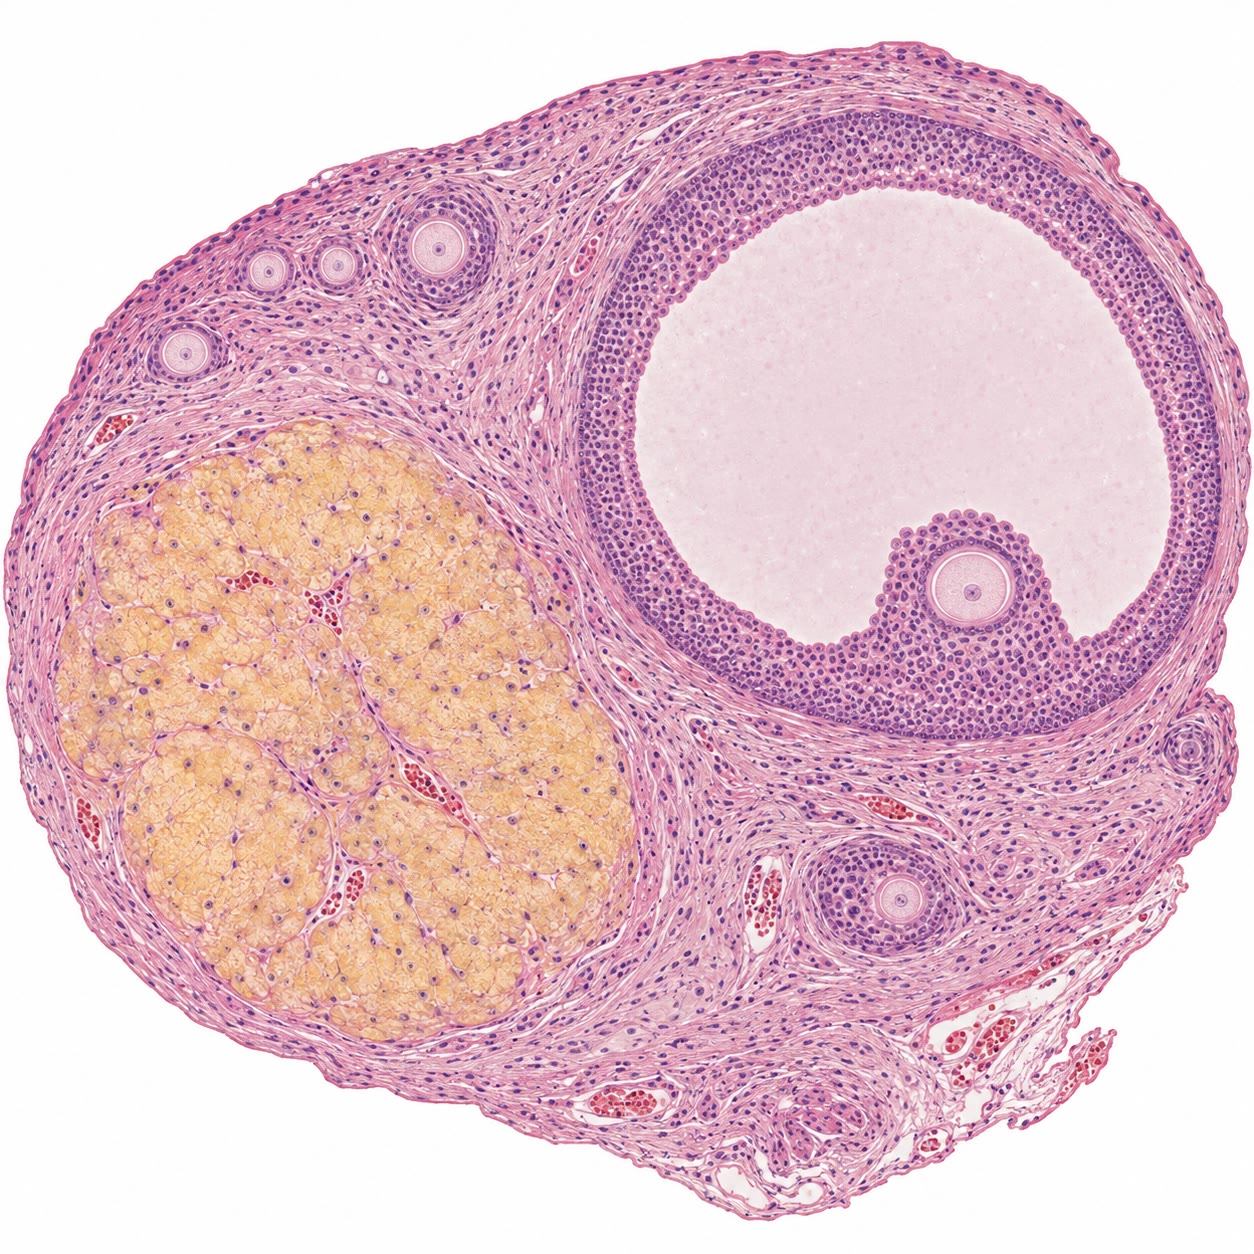
\includegraphics[width=0.46\linewidth]{images/book4/ai/b4-09-ovary-histology.jpg}

{\small 卵巢切片：成熟\omterm{def:b2:mammal-reproduction:ovary}{卵泡}及其腔、卵母细胞，
表层下的小原始\omterm{def:b2:mammal-reproduction:ovary}{卵泡}，以及前一周期遗留的
\omterm{def:b2:mammal-reproduction:ovary}{黄体}。}
\end{omfigure}

\begin{theorem}[从负反馈到正反馈的转换]\label{thm:b2:reproductive-hormones:switch}
\index{正反馈!LH 峰}
\omterm{def:b2:mammal-reproduction:ovary}{卵泡}早期雌二醇水平较低时，
抑制 LH 和 FSH；雌二醇高于约 \qty{200}{pg/mL}，并维持
超过约 \qty{36}{h}，则产生相反的作用：促使
下丘脑释放一阵 GnRH，垂体对此作出反应，
LH 升高约十倍。这一机制改变的是作用方向，而非
强度：高而持续的剂量在垂体中诱导
大量 LH 储备，并提高对 GnRH 的敏感性；在下丘脑中
（通过 kisspeptin 神经元）使 GnRH
脉冲发生器切换为峰值模式。这一转换把分级
信号——\omterm{def:b2:mammal-reproduction:ovary}{卵泡}产生多少雌二醇——变为
按日期定时的全或无事件，这正是\omterm{def:b2:mammal-reproduction:ovary}{排卵}
所需要的；又因为只有成熟的大\omterm{def:b2:mammal-reproduction:ovary}{卵泡}才能维持
\qty{200}{pg/mL}，峰值只在有卵子待排出时才会出现。
\omterm{def:b2:mammal-reproduction:ovary}{排卵}之后，\omterm{def:b2:mammal-reproduction:ovary}{黄体}分泌的
孕酮恢复负反馈，
不再出现第二次峰值。
\end{theorem}
\begin{proof}[证据]
在下丘脑—垂体轴被抑制的女性和猴子中，输注
雌二醇使血浆水平升至 \qty{200}{pg/mL} 以上并持续
两天，随后出现 LH 峰；同等剂量只给予一天，
或较低水平持续三天，则不出现。输注前给予孕酮
会阻断峰值；同时给予则使之提前
并增强之。剂量和持续时间的阈值再现了
自然雌二醇上升所引起的自然峰值的时间。
\end{proof}

\section{超越周期的调控}

\begin{proposition}[妊娠、泌乳与绝经]\label{prop:b2:reproductive-hormones:overrides}
\index{人绒毛膜促性腺激素}\index{绝经}
\omterm{def:b2:mammal-reproduction:implantation}{着床}的胚胎分泌 \emph{hCG}，这是一种类 LH 激素，
与 LH 受体结合，使\omterm{def:b2:mammal-reproduction:ovary}{黄体}保持存活并
持续分泌至第十四天之后；到第十周时，\omterm{def:b2:mammal-reproduction:placenta}{胎盘}自身
即可分泌足够的孕酮和雌激素以维持妊娠，
\omterm{def:b2:mammal-reproduction:ovary}{黄体}便不再必需。整个妊娠期间，高水平的类固醇
使 LH 和 FSH 保持为零：没有\omterm{def:b2:mammal-reproduction:ovary}{卵泡}生长，
也不\omterm{def:b2:mammal-reproduction:ovary}{排卵}。分娩后，哺乳会升高\omterm{prop:b2:mammal-reproduction:lactation}{催乳素}并减缓 GnRH
脉冲，\omterm{def:b2:mammal-reproduction:ovary}{排卵}被抑制长达数月。在
\emph{\omterm{prop:b2:reproductive-hormones:overrides}{绝经}}时，\omterm{def:b2:mammal-reproduction:ovary}{卵泡}库耗尽：雌二醇和
抑制素下降，由于缺少反馈，LH 和 FSH 升至
先前水平的十倍并维持于此——这是一个
已停止应答的腺体的特征。
\end{proposition}

\begin{proposition}[避孕与辅助生殖]\label{prop:b2:reproductive-hormones:clinic}
\index{避孕!激素}\index{体外受精}
复方口服避孕药每天提供一种合成雌激素和一种孕激素：
恒定的类固醇水平使 FSH 和 LH 保持较低，没有
\omterm{def:b2:mammal-reproduction:ovary}{卵泡}被募集，不出现雌二醇上升，峰值
也就不会出现；孕激素还会使宫颈黏液变稠。
七天停药期让\omterm{def:b2:reproductive-hormones:cycle}{子宫内膜}出血；漏服药片超过
连续两天，FSH 便会逃逸，\omterm{def:b2:mammal-reproduction:ovary}{卵泡}可能生长。
紧急避孕可在数天内推迟峰值，所用为
大剂量孕激素。在\emph{\omterm{prop:b2:reproductive-hormones:clinic}{体外受精}}中，下丘脑—垂体轴
被反向驱动：连续十天每日给予 FSH，压制
单一优势\omterm{def:b2:mammal-reproduction:ovary}{卵泡}的选择，使十个或更多\omterm{def:b2:mammal-reproduction:ovary}{卵泡}成熟；
GnRH 拮抗剂防止过早的自发峰值；注射
hCG 替代峰值，卵母细胞在 34
至 36 小时后采集，恰好早于它们本应排出的时刻；
卵子在培养皿中受精，移植一至两个胚胎，
其余冷冻保存。在男性中，外源睾酮或 GnRH 类似物
通过抑制 LH 来抑制\omterm{def:b2:mammal-reproduction:testis}{精子发生}——这是一种
男性激素避孕药的原理，目前尚未上市。这一切都是
第一节中的轴反过来读。
\end{proposition}

\section{练习}

\begin{exercise}[$\star$]\label{exo:b2:reproductive-hormones:1}
画出男性的轴：三个层级、四种激素、
两条反馈回路，以及每种激素作用的细胞。
\end{exercise}

\begin{exercise}[$\star$]\label{exo:b2:reproductive-hormones:2}
给出卵巢周期和子宫周期的各个时期及其天数，
并说明每个时期占主导的激素。
\end{exercise}

\begin{exercise}[$\star$]\label{exo:b2:reproductive-hormones:3}
解释复方口服避孕药如何抑制\omterm{def:b2:mammal-reproduction:ovary}{排卵}，以及
为何在停药周会出血。
\end{exercise}

\begin{exercise}[$\star$]\label{exo:b2:reproductive-hormones:4}
去势的成年男性体内 LH、FSH 及第二性征会
发生什么变化？注射的睾酮能逆转其中哪些，
不能逆转哪些？
\end{exercise}

\begin{exercise}[$\star\star$]\label{exo:b2:reproductive-hormones:5}
在\omterm{def:b2:reproductive-hormones:cycle}{卵泡期}，GnRH 脉冲每 \qty{90}{min} 出现一次，
在\omterm{def:b2:reproductive-hormones:cycle}{黄体期}每 \qty{4}{h} 出现一次。两个时期每天各有多少次脉冲？
垂体在快速脉冲下倾向于分泌 LH，在慢速脉冲下倾向于分泌 FSH：
\omterm{def:b2:mammal-reproduction:ovary}{黄体}退化时，哪种促性腺激素应首先升高，
以及为什么它是正确的那一种？
\end{exercise}

\begin{exercise}[$\star\star$]\label{exo:b2:reproductive-hormones:6}
将 \qty{200}{pg/mL} 的氧雌二醇（摩尔质量
\qty{272}{g/mol}）换算为 \unit{pmol/L}，并将 \qty{15}{ng/mL} 的
孕酮（\qty{314}{g/mol}）换算为 \unit{nmol/L}。
在\omterm{def:b2:mammal-reproduction:ovary}{排卵}峰阈值时，每微升血浆中有多少个
氧雌二醇分子？
\end{exercise}

\begin{exercise}[$\star\star$]\label{exo:b2:reproductive-hormones:7}
某女性的\omterm{def:b2:reproductive-hormones:cycle}{月经周期}为 35 天。已知\omterm{def:b2:reproductive-hormones:cycle}{黄体期}长度固定，
她在哪一天\omterm{def:b2:mammal-reproduction:ovary}{排卵}？若精子存活三天、卵子存活一天，
哪些天为易受孕期？
为什么日历法对周期不规则者失效？
\end{exercise}

\begin{exercise}[$\star\star$]\label{exo:b2:reproductive-hormones:8}
一个胚胎在 28 天周期的第 21 天\omterm{def:b2:mammal-reproduction:implantation}{着床}，其 hCG 起始为
\qty{1}{IU/L}，每两天翻一番。\omterm{def:b2:mammal-reproduction:ovary}{黄体}需要
在第 26 天前获得数个 IU/L 的 hCG 才能存活。该胚胎是否及时\omterm{def:b2:mammal-reproduction:implantation}{着床}？
若\omterm{def:b2:mammal-reproduction:implantation}{着床}推迟至第 25 天，会发生什么？
\end{exercise}

\begin{exercise}[$\star\star$]\label{exo:b2:reproductive-hormones:9}
说明 Knobil 实验显示了什么、排除了什么，
并预测给予女性长效 GnRH 激动剂一个月后，
LH、氧雌二醇和\omterm{def:b2:reproductive-hormones:cycle}{子宫内膜}分别会发生什么变化。
\end{exercise}

\begin{exercise}[$\star\star\star$]\label{exo:b2:reproductive-hormones:10}
在受体模型中，取每小时 $s = 100$ 个受体，$d =
\qty{0.5}{h^{-1}}$，且有激素存在时 $iH = \qty{6}{h^{-1}}$，
分别计算无激素时与持续给予激素时的稳态受体数。
若每小时给予一次两分钟的脉冲，计算每次脉冲损失的受体数，
以及下一次脉冲前已恢复的亏损比例，
并推断受体池最终稳定所围绕的
水平。
\end{exercise}

\begin{exercise}[$\star\star\star$]\label{exo:b2:reproductive-hormones:11}
一名\omterm{prop:b2:reproductive-hormones:overrides}{绝经}后女性的 LH 和 FSH 为年轻女性的十倍，
氧雌二醇极低；一名分泌\omterm{prop:b2:mammal-reproduction:lactation}{催乳素}的垂体肿瘤女性，
LH 低、氧雌二醇低且无\omterm{def:b2:reproductive-hormones:cycle}{月经周期}；一名颗粒细胞瘤女性，
氧雌二醇高、LH 低且无\omterm{def:b2:reproductive-hormones:cycle}{月经周期}。请从下丘脑–垂体–性腺轴出发，
分别解释每种特征。
\end{exercise}

\begin{exercise}[$\star\star\star$]\label{exo:b2:reproductive-hormones:12}
“同一种激素先抑制、后诱发 LH 峰。”
请解释氧雌二醇如何兼具两种作用，为什么\omterm{def:b2:mammal-reproduction:ovary}{排卵}需要的是开关，
而非调节旋钮，以及若用调节旋钮会出现什么问题。
\end{exercise}

\section{问题：一个被测量的周期}

\begin{problem}[{周末问题——读取一个周期的每日激素测量数据，
读出其各阶段、排卵日与易受孕期；计算排卵峰阈值、
黄体的时钟与 hCG 挽救；用受体模型解释 Knobil 实验；
并从临床角度逆向驱动该轴，
最终求出排卵日、
黄体期长度、易受孕期与排卵峰阈值}]
\label{pb:b2:reproductive-hormones:1}
对某女性周期中选定的若干天采血，结果如下：

\begin{center}
\small
\begin{tabular}{lcccccccccc}
\hline
天 & 1 & 5 & 8 & 11 & 12 & 13 & 14 & 15 & 21 & 27 \\
\hline
氧雌二醇（\unit{pg/mL}） & 40 & 60 & 110 & 210 & 260 & 310 & 220 & 150 & 160 & 50 \\
LH（\unit{IU/L}） & 5 & 5 & 6 & 7 & 8 & 20 & 65 & 15 & 4 & 4 \\
孕酮（\unit{ng/mL}） & 0.5 & 0.5 & 0.6 & 0.7 & 0.8 & 1.0 & 1.5 & 3 & 16 & 2 \\
体温（\unit{\celsius}） & 36.4 & 36.4 & 36.4 & 36.4 & 36.4 & 36.4 & 36.4 & 36.5 & 36.8 & 36.7 \\
\hline
\end{tabular}
\end{center}

月经分别于第 1 天和第 29 天开始。

\medskip
\noindent\textbf{第一部分——读取周期。}
\begin{enumerate}
  \item 根据表格，指出\omterm{def:b2:reproductive-hormones:cycle}{卵泡期}与\omterm{def:b2:reproductive-hormones:cycle}{黄体期}，
        以及标志各阶段的激素。
  \item LH 峰值出现在哪一天？\omterm{def:b2:mammal-reproduction:ovary}{排卵}发生在哪一天？
  \item \omterm{def:b2:reproductive-hormones:cycle}{黄体期}持续多长时间？
        这是否与\omterm{def:b2:mammal-reproduction:ovary}{黄体}的寿命相符？
  \item 解释体温的变化，以及为何它能证实\omterm{def:b2:mammal-reproduction:ovary}{排卵}，
        却不能预测\omterm{def:b2:mammal-reproduction:ovary}{排卵}。
  \item 氧雌二醇高于 \qty{200}{pg/mL} 是在哪些天？
        并说明其持续时间与 LH 峰的关系。
  \item 求出本周期的易受孕期（精子存活三天，卵子
        存活一天）。
\end{enumerate}

\medskip
\noindent\textbf{第二部分——数值计算。}
\begin{enumerate}[resume]
  \item 将第 13 天的氧雌二醇换算为 \unit{pmol/L}，并将
        第 21 天的孕酮换算为 \unit{nmol/L}。
  \item LH 从第 12 天到第 14 天升高了多少倍？
        此后其下降为何如此迅速（LH 的半衰期
        约为 \qty{1}{h}）？
  \item 若该女性下一周期的\omterm{def:b2:reproductive-hormones:cycle}{卵泡期}为 21 天，
        她将在哪一天\omterm{def:b2:mammal-reproduction:ovary}{排卵}，周期长度
        又为多少？
  \item 胚胎在\omterm{def:b2:mammal-reproduction:ovary}{排卵}后 7 天\omterm{def:b2:mammal-reproduction:implantation}{着床}。hCG 会在本周期的哪一天出现，
        若其从 \qty{1}{IU/L} 开始、每两天翻一番，
        则到第 27 天时将达到多少？
  \item 说明第 27 天孕酮为 \qty{2}{ng/mL} 这一结果为何表明
        未发生胚胎\omterm{def:b2:mammal-reproduction:implantation}{着床}。
  \item 若曾有胚胎\omterm{def:b2:mammal-reproduction:implantation}{着床}，第 27 天的孕酮和氧雌二醇值
        应分别是多少？
\end{enumerate}

\medskip
\noindent\textbf{第三部分——反馈与脉冲。}
\begin{enumerate}[resume]
  \item 结合反馈的符号，解释周期开始时 FSH 为何最高，
        以及为何通常只有一个\omterm{def:b2:mammal-reproduction:ovary}{卵泡}
        能够存活。
  \item 在受体模型中，取 $s = 100$ 每小时，$d =
        \qty{0.5}{h^{-1}}$，$iH = \qty{6}{h^{-1}}$，计算
        无激素时及持续激素作用下的 $R^*$。
  \item 一次脉冲持续 \qty{2}{min}。从未受刺激时的
        $R^*$ 出发，一次脉冲使受体数减少多少（用线性近似
        $iHR\,\Delta t$）？
        下一次脉冲前的一小时内，亏损中哪一部分得以恢复
        （时间常数为 $1/d$）？池中数量大约稳定在
        何种水平？
  \item 利用这些数值，解释 Knobil 的实验结果。
  \item 一名男性因前列腺癌持续接受 GnRH 激动剂治疗，
        预测用药一天后及一个月后其 LH 与睾酮的水平，
        并解释二者的差异。
  \item 一名女性的颗粒层细胞不能合成抑制素，预测其
        FSH 和 LH 水平，以及对\omterm{def:b2:mammal-reproduction:ovary}{卵泡}募集的后果。
\end{enumerate}

\medskip
\noindent\textbf{第四部分——临床应用。}
\begin{enumerate}[resume]
  \item 对该女性进行\omterm{prop:b2:reproductive-hormones:clinic}{体外受精}，自第 2 天起每天注射 FSH，
        解释为何十个\omterm{def:b2:mammal-reproduction:ovary}{卵泡}而非一个\omterm{def:b2:mammal-reproduction:ovary}{卵泡}成熟。
  \item 为何自第 6 天起加入 GnRH 拮抗剂，
        若不加入，会发生什么？
  \item \omterm{def:b2:mammal-reproduction:ovary}{卵泡}成熟时注射 hCG；卵母细胞在
        注射后 35 小时被采集。请根据表格说明该时间安排的依据。
  \item 采集到十个卵母细胞，其中 \qty{70}{\%} 受精，
        \qty{40}{\%} 的胚胎发育至\omterm{def:b2:mammal-reproduction:implantation}{囊胚}期，每个移入的\omterm{def:b2:mammal-reproduction:implantation}{囊胚}
        以 $0.35$ 的概率\omterm{def:b2:mammal-reproduction:implantation}{着床}。
        \omterm{def:b2:mammal-reproduction:implantation}{囊胚}的期望数是多少？移入两个\omterm{def:b2:mammal-reproduction:implantation}{囊胚}时，
        至少一次妊娠的概率为多少？
  \item 解释该女性服用复方避孕药时，
        为何所得表格中没有 LH 峰，
        也没有孕酮上升。
  \item 以 GnRH 拮抗剂为基础的男性避孕药同样会消除睾酮，
        应与之同时给予何种物质？为何给予该物质
        仍无法恢复精子的产生？
  \item 给出结果：\omterm{def:b2:mammal-reproduction:ovary}{排卵}日、\omterm{def:b2:reproductive-hormones:cycle}{黄体期}长度、可育窗，
        以及引发 LH 峰的雌二醇阈值
        与持续时间。
\end{enumerate}
\end{problem}
